\chapter{Evaluation and Discussion}
\section{Confusable Domains}
\subsection{Identification and Examples of Targeted Domains}

The choice of such domains to target and outsource depends on many factors, each with its implications on the business strategy, marketing, and observance by law. The selection of these domains hence matters a lot in creating potential conflict especially those related to existing trademarks. Understanding these selection criteria is very important to try to negotiate the hurdles of the digital market and to protect rights through intellectual property. 

To navigate these complexities effectively, it is essential to consider several key factors. 

\begin{itemize}
  \item \textbf{Commercial Appeal:} High commercial appeal domains are lucrative targets due to the extremely high possibility of attracting a large traffic flow, with potential revenue generation and used for blackmailing purposes in which they demand payment to relinquish the domain. Such names are easy to remember, short in length, and directly linked to products or services under some category that is searched most frequently.\cite{Li2002ConflictDomainTrademark}
  
  \item \textbf{Keyword Relevance:} Targeted domains have a certain relevance that holds the keyword itself. These domains are ranked higher in search engine outputs and attract organic traffic, making them a useful tool for businesses aiming to align with the primary keywords used by their target customers in which they are targeted becasue they generate huge amount of clicks.
  
  \item \textbf{Similarity to Well-known Trademarks:} This refers to the practice of registering domains that are similar or confusingly like existing trademarks known as cybersquatting. This can lead to confrontations with the rightful trademark holders. Trademark law aims to prevent consumer confusion and protect the goodwill associated with the trademark, particularly in disputes over domain infringement.
\end{itemize}

\subsection{Real-life examples}

\begin{itemize}
    \item \textbf{Cybersquatting :} is securing domain names that are the same as or in the likeness of trademarks or brand names, with the intent to sell them at grossly marked-up prices back to the target , showing ads which bad actors benefit financially from clicks generated by users who visit the site expecting it to be associated with the target , harvesting emails and redirecting to malicious websites.Perhaps the best example in that respect was one of the largest dairy product companies in India, Amul. In the financial year of 2019-2020, the turnover that was brought into account through Amul was staggering, to say the least. During this period, the company was a target for cybersquatting, where some bad actors had registered similar domains impersonating as Amul. These had been used for constructing several phishing sites to further various fraudulent schemes like solicitation for payments under the pretext of distributorship of Amul products and also of securing jobs in Amul. This operation which was active between 2018 and 2020 then finally came down to a public warning and further law actions by Amul to deal with fraudulent activities happening under these domains. Such abuses in the domain name system expose even long-established brands to threats and show the relevance of legal action and public-awareness activities for resolving them. \cite{MehtaCybersquatting}
    
    \item \textbf{Typosquatting- URL hijacking :} it deals with the registration of misspelled variants of well-known domain names for the mere purpose of capturing traffic from users who tend to make mistakes in typing a URL. They could register "goggle.com" instead of "google.com" which was used to direct users to a site that bombarded their browsers with pop-ups and ads , leading to malware infections as that site was designed to capitalize on accidental misspellings or phishing  attempts that tricked users into visiting. \cite{SplunkTyposquatting} An example in December 2020, US healthcare provider Elara Caring suffered a major cyber incident that brought into sharp perspective the vulnerabilities lying at the heart of healthcare's cybersecurity framework. The incident was initiated by gaining unauthorized computer access to email accounts of its staff and resulted in personal data breaches for more than 100,000 elderly patients. Compromised information included almost every variety of personally identifiable data, from their financial details through to Social Security numbers. The attacker, despite being detected, remained in the system for a week, which may be a signal that the incident response could be better. \cite{PandaSecurityPhishing}
    
     \item \textbf{Reverse Domain Name Hijacking  :} is the act of trademark owners trying to take a domain away from its rightful holder based on the claim of trademark rights, considering that he holds a bona fide registration over the said domain. It may otherwise be described as using legal or dispute resolution mechanisms to try to force people from their domains. \cite{Sun2006DomainTrademarkConflict}

    An RDNH was claimed in a UDRP action against "groovle.com," in which the domain was purported to be too close to Google's trademark. However, since the domain was used for another search engine, it was deemed legitimately used and not to have infringed on Google's trademark or registered in bad faith. \cite{Singh2011ReverseDomainHijacking}
\end{itemize}


\subsection {Homograph attacks} 

The threat of a homograph based attack weaponizing visually similar characters to swindle people persists. This is also true when attackers register domain names to appear like reputable ones, such as when the Latin letter 'l' ( lower case "el") is visually confusable with the Latin latter with 'I' ( upper case eye ), and so on. Such as http://www.paypal.com vs http://www.paypaI.com.  Latin character homographs were traditionally used up to now, though with the advent of International Domain Names there are so many more possibilities. Although this rising trend suggests a higher potential for such attacks, current data says they are not very prevalent. Vigilance is, however, important because of the increasing trend in phishing incidents and the ease with which users can be diverted to suspicious sites.

For example, a new study measures homograph attacks on internet users: "Cutting through the Confusion" explains the growth and potential impact of such attacks. \cite{holgers2006homograph} The current study tries to measure how attackers are able to register domain names having visual similarity with respect to those which are legitimate and authoritative by using confusable characters during phishing. These confusable characters, though seemingly similar to the letters in the authoritative domains, are actually characters different from one another or come from multiple scripts like Cyrillic or Greek, represented in web browsers using punycode to keep a consistent user experience. This study is summarized in a table of the possible confusable domain names, the count of the actual number of the confusable domain names they found available, and the authoritative domains' names. For example, 'yahoo.com' has more than 5000 possible confusables but has been registered two. Another instance is 'google.com', with a thousand possible confusables yet was registered 4. These confusable domains often contain punycode in their web address, which is not immediately recognized at the first glance by the average user.

This table will be added below in order to clearly show, by means of a graphic illustration, the scope and scale of homograph attacks, which point to the potential risks that these attacks could pose to online security and the awareness and mitigation strategies that need to be put in place for protecting internet users from such deceptive practices. Its noteworthy contribution will be added to the body of knowledge about how homograph attacks are leveraged and their prevalence across various high profile domains.



\captionsetup{font= footnotesize}
\begin{figure}[H]
    \centering
    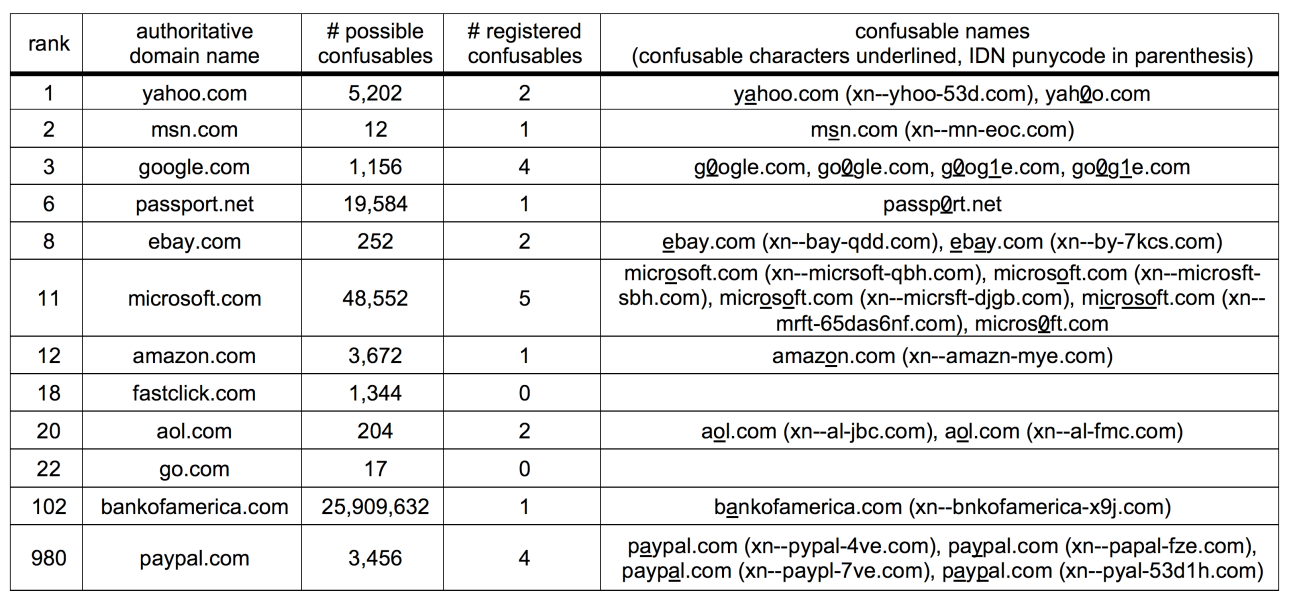
\includegraphics[width=1\linewidth]{evaluation/confusable.png}
    \caption{Registered confusables for popular domains}
    \label{fig:figureAlot1}
\end{figure}

\subsection{ Real-life Mitigations}

The following scenarios are examples of real-life confusable domain mitigations :

\begin{itemize}
    \item \textbf{Cloudflare's Zero Trust Services Approach :} Protection from this problem of newly created phishing websites is given by Cloudflare itself with its protection in the form of Zero Trust services, finding these websites, and blocking confusable domains. Cloudfare zero-trust rules can be enforced using Cloudfare Gateway in a way that they deny access to these illegitimate domains. In such a way, corporate networks are supposed to be secured from phishing attempts that take advantage of human trust in well-known brands \cite{Cloudflare2023}. Cloudflare's Zero Trust services enable a proactive approach to blocking confusable domains, which are important to avoid serving phishing sites. In particular, this mitigating measure will be triggered on the first query that involves any domain that is made through the 1.1.1.1 DNS resolver. Such queries will be inspected by the system and checked against a list of possible phishing domains through a “fuzzy” matching protocol. If the domain matches any of the saved patterns for legitimate brands, then Cloudflare's service would throw an alert. This method used by the server ensures that any domain trying to impersonate a known or respectable brand is detected as soon as it happens in which it provides both real-time monitoring and the capability to search into a historical archive of those domain names, by notifying a security team about new domains observed during the last 30 days that match their saved patterns. This enables a direct review and instant additional taking actions by this domain. The system can also be utilized by Cloudflare for special investigation in a one-time domain hunt for some specific domain or pattern, which might become potentially dangerous from a security point of view.

     \item \textbf{IDN Handling of Google Chrome: } Google Chrome enforces an IDN (Internationalized Domain Names) policy to determine which form the Unicode or punycode form a domain label should be displayed in. The domain label is tested to determine whether it has mixed script, invisible characters, or visually confusable characters, and whether it is actually validly converted to Unicode. For instance, domains containing characters of different scripts, or those that are clearly identified as mixed script confusables, will be displayed in punycode, warning the users of potential deceptions. Chrome further offers comprehensive warnings to secure URLs that appear to be an imitation of already known web pages. \cite{ChromiumIDN}
     
\end{itemize}

In addition to what I mentioned above, let us look at the most popular mitigations used world-wide :

\begin{enumerate}
 
  \item Typo-squatting Detection Tool: Tools such as DNStwist and URLCrazy are used to offer organizations similar domain names so that they can either secure these domain names in advance or file litigation for the same.
  \item Anti-Phishing Working Group (APWG): It is a pool for stakeholders to share intelligence, trends and best practices regarding phishing and similar threats associated with confusable domains in which mitigation is carried out in collaboration action between cybersecurity entities and domain registrars, as it allows sharing of threat intelligence with respect or cancelling out the holding of malicious domains.
\end{enumerate}

\subsection{Collaboration Among Registrars, Registries, and DNS Collaborators}

This collaboration should be achieved with DNS registry, registry and collaborators. In that way, they can boost common resources and intelligence that can guide in making the internet more secure and resilient. This strictly falls within the remit of registries and registrars acting in collaboration to put in place such stringent registration policy with procedures for verification, checking against mimicking existing trademarks or even popular domain names.

In this way, the collaboration can even manifest itself via the sharing of sensitive data with regards to domain abuse threats and trends. Databases and threat intelligence platforms are shared amongst stakeholders, allowing them to anticipate and avert most such perils well before they impact netizens. This collective effort will enable the formulation of standards by which to coordinate responses to confusable domain incident reports. Mitigating confusable domains demands that registrars, registries, and DNS collaborators work in a common effort. This is due to the increasing level of threats and the shared responsibility of all the actors involved in the DNS ecosystem. \cite{Catania2022} To put this into perspective, here are some examples: 




\begin{enumerate}
  \item Recent changes in the contract from ICANN's contracted parties have imposed on registrars and registries new specifications to define DNS abuse, together with clear requirements for the actions to be taken by such parties immediately actionable evidence of abuse is received. This is a major step towards establishing more clarity about the roles that may be played by these different stakeholders in addressing the matter of DNS abuse and ensuring there is a common approach to redress. \cite{Weinstein2023}
  \item Approved new obligations of ICANN's contracted parties have been by the community itself further to mitigate DNS abuse, thereby demonstrating the will of the community to come together to address the issues of DNS abuse. \cite{ICANN2023}
  \item Efforts like NetBeacon, with the support of the DNS Abuse Institute, are being rolled out to reduce friction in reporting and mitigating DNS abuse. This service solves the current complexities and quality standards associated with the reporting of DNS abuse as it makes the work easier for the registrars, ultimately narrowing down their scope to the relevant and evidenced report as well as it underlines the need for cooperation among registrars, registries, and other DNS stakeholders. This is what is capable of saving the Internet and safeguarding at the same time the credibility and confidence of DNS. \cite{NetBeacon}
  
\end{enumerate}

Real-life examples of entities seeking to block the resolution of DNS names, especially in connection with public recursive DNS servers, frequently revolve around matters of control, filtering, or securing internet traffic with various kinds of motivations corresponding to such sectors. Some attempted these efforts at the governmental, corporate, and individual levels. As typical examples that pinpoint those instances, consider:

\begin{enumerate}
    \item Governmental Efforts to Block DNS Resolutions : Governments may interfere directly in the DNS operation to enforce some censorship or block access to particular types of content. For instance, China uses the Great Firewall for regulation concerning access to the World Wide Web within their territory, including doing some mishandling connected with the DNS in order to block out unwanted content. \cite{XuAlbert2017MediaCensorship}
    \item Corporate and ISP DNS Filtering : DNS filtering can be deployed by companies and even ISPs in a bid to achieve enhanced online security. For instance, Heimdal Security explicates how the DNS filtering works as one of the measures for preventing their access to various harmful or inappropriate websites since it first checks the requests for domains. If some are actually flagged, access is denied, hence maintaining both security and productivity within one's organization. This approach is really very effective for the prevention of phishing and malware attacks because it stops the DNS requests towards the malicious sites. 
    \item Ad Block DNS Services :  Cloudflare discusses how DNS filtering can be used to prevent access to malicious sites and also filter what is harmful or unfit for viewing. This is done at the DNS level so as to prevent these sites from loading on devices. Cloudflare uses its DNS to filter part of a more prominent policy of access control—an effort to secure company data and govern what employees will see on the network they manage.    
\end{enumerate}

 On the negative side, attackers are taking advantage of DNS blocking mechanisms to perform DNS-based attacks. These include using DGAs (Domain Generation Algorithms) for malware communication, using FastFlux techniques for slipstreaming attacks, basically creating malicious newly registered domains (NRDs) that appear benign and legitimate to an outside observer, etc. All this makes it difficult to block bad content at the level of DNS, which calls for quite sophisticated countermeasures.


\subsection{Techniques for Mitigating Confusable Domains}

Mitigating confusable domains requires sophisticated techniques tailored to address the unique challenges presented by both non-Internationalised Domain Names (non-IDNs) and Internationalized Domain Names (IDNs). This differentiation is significant  due to the distinct nature of threats they pose and the technical feasibility of the mitigation strategies applicable to each. The following is a detailed examination of mitigation techniques, along with discussions of the operational feasibility and potential collaboration frameworks involved.

Non-IDNs Mitigation Techniques : Strategies focus on identifying and mitigating domain squatting and typo-squatting, where attackers register domains that are typographical errors or close variants of legitimate domains to deceive users.

\begin{enumerate}
  \item Registry-Level Measures: Domain registries can implement checks to prevent the registration of domains that are similar to the existing trademarks or brand names, using algorithms to detect variations and misspellings closely resembling protected names. \cite{WTR2020} 
  \item Trademark Protection Programs: Services like the Trademark Clearinghouse (TMCH) offer mechanisms for trademark holders to protect their rights by receiving notifications when someone attempts to register a domain matching their trademark. \cite{ICANNTMCH}
  \item Automated Monitoring and Reporting: Automated systems can continuously monitor domain registrations for names that closely resemble known trademarks or brand names, enabling rapid detection and legal action against infringers. \cite{TMCH2023}
\end{enumerate}

IDNs Mitigation Techniques : The challenge with IDNs lies in the potential for homograph attacks, where attackers use characters from different scripts that appear visually like characters in the Latin script to create deceptive domains.

\begin{enumerate}
  \item Punycode Awareness and Monitoring: Web browsers and security tools convert IDNs to punycode, a representation that encodes the Unicode characters in ASCII. Awareness of punycode and monitoring for suspicious registrations can help identify potential homograph domains. \cite{SOCRadar2023}
  \item Browser-Level Defenses: Modern web browsers have implemented defences against IDN homograph attacks by displaying the punycode version of the domain or alerting users when a domain name contains characters from multiple scripts. \cite{Malwarebytes2017}
  \item Collaborative Blacklisting and Sharing of Threat Intelligence: Organisations can collaborate to share intelligence about known malicious IDNs, contributing to comprehensive blacklists that can be used by registrars, DNS providers, and end-users to block access to malicious sites. \cite{CyberThreatAlliance2023}
  
\end{enumerate}


However, ICANN plays a pivotal role in the detection of confusable domains as it detects confusable domains, especially with respect to Internationalized Domain Names (IDNs) but also it doesn't provide a direct list publication on confusable domain, just like the other gTLD registries. Instead, they tend to develop the frameworks and guidelines for managing the threats related to IDNs and name collisions. This will involve the development of protocols regarding how the processing of internationalized domain names would be done and how the impact that name collisions may possibly have on the domain name system is minimized. \cite{ICANNIDNs}

People detect on-Internationalized Domain Names (non-IDNs) and Internationalized Domain Names (IDNs) using comprehensive domain, IP, and DNS intelligence tools. Tools which can do so, such as those offered by services like the WhoisXML API, help check domain names for the presence of suspiciously similar domains that could potentially confuse or deceive consumers. An IDN deceptive score is given by means of an algorithm to such types of domains that take into account visual similarities, brand names, and TLD features to see if a domain name is being prepared for deceptive purposes. This approach has proven to be effective in academic research projects at identifying deceptive IDNs over millions of domains distributed across various top-level domains. \cite{WhoisXMLAPI}

\subsection{Technical and Operational Feasibility}
The technical feasibility of these techniques varies. Registry-level measures and trademark protection programmes are quite effective, but require cooperation and standardisation across different legal jurisdictions. Automated monitoring is technically feasible and can be implemented on a scale but requires resources for continuous operation and legal follow-up. Browser-level defences are among the most directly impactful, protecting users at the point of access, yet they depend on browser vendors' willingness to implement and maintain these features, and collaboration frameworks play a crucial role in mitigating confusable domains. Initiatives such as the Trademark Clearinghouse (TMCH) facilitate cooperation between trademark holders and domain registries. Meanwhile, organisations such as the Anti-Phishing Working Group (APWG) and the Internet Corporation for Assigned Names and Numbers (ICANN) work toward broader solutions that encompass both non-IDNs and IDNs.

\subsection{ Transparency in Mitigation Efforts}

Transparency in the mitigation of confusable domains plays a pivotal role in the broader strategy to secure the Internet against phishing attacks, trademark infringement, and other malicious activities. This concept entails the practices adopted by domain registries and registrars in identifying potentially malicious domains that mimic or closely resemble legitimate ones, and the extent to which these entities disclose identified confusable domains to the public. One of the primary methods to improve transparency involves the publication of lists of confusable names by registries and registrars. These lists typically include domains flagged for their similarity to existing domain names, potentially infringing trademarks, or those that could be used for malicious purposes. The publication aims to alert the internet community, including businesses and end-users, about possible threats, thereby fostering a proactive approach to domain name security. Here is how transparency can be applied to each of the mitigation techniques described:

\begin{itemize}
  \item \textbf{Cloudflare's Zero Trust Services Approach: }Cloudflare's process for identifying and blocking confusable domains should be transparent to its users. This includes detailing the criteria for flagging domains as phishing sites and the mechanisms in place for users to appeal or request a review of blocked domains. By openly sharing the methodology behind their zero-trust rules and how they are applied through the Cloudflare Gateway, trust in Cloudflare's protective measures is bolstered among corporate networks.
  
  
  \item \textbf{IDN Handling of Google Chrome:} Google's approach to displaying domain names in Unicode or punycode based on their potential for deception benefits from transparency about its IDN policy. Detailed explanations of the checks performed (e.g., mixed script detection, invisible characters) and how decisions are made improve user understanding and awareness of potential threats. Furthermore, publishing information on how users can report misclassified domains or suggest improvements to the IDN policy can further empower users and foster a safer Internet environment.
  
  
  \item \textbf{Typo-squatting Detection Tools: }The effectiveness of tools like DNStwist and URLCrazy in helping organizations identify potential confusable domains relies on transparency about how these tools generate similar domain names and the criteria used for detection. Openly sharing updates, methodologies, and case studies can help organisations better understand how to use these tools proactively.
  
  \item \textbf{Collaborative Efforts and Intelligence Sharing: }The partnership between cybersecurity entities and domain registrars, as well as initiatives such as the Anti-Phishing Working Group (APWG), should prioritise transparency in their operations. This includes the sharing of methodologies for threat detection, the criteria for taking action against malicious domains, and the processes for stakeholders to contribute or access shared intelligence. Transparency in these collaborative efforts ensures that actions taken against confusable domains are fair, understood by all parties involved, and supported by a broad community of internet security stakeholders.
  
 \item \textbf{Transparency for non-IDN registries : } 

 \begin{enumerate}
  \item Registry-Level Measures: Transparency in level-registry measures becomes a necessity if trust has to be kept between registrants and domain trademark owners. They are published criteria and algorithms used to find variations and misspellings of the names submitted for protection. Making these publicly available can then ensure fairness and feedback in detecting mechanisms is therefore paved for improving them.
  \item Trademark Protection Programs: Services such as those from a Trademark Clearinghouse (TMCH) should operate with full transparency regarding the conductance of verification, matching, and notification. This can help trademark holders by demonstrating transparent guideline procedures that show both the rights of trademark holders and what needs to be done to effectively protect their brands.
  \item Automated Monitoring and Reporting: The automated monitoring systems must be built with such predefined criteria, algorithms, and thresholds that potentially support the involvement of stakeholders. It also makes sure that the brand owners are aware to what extent his trademarks are protected, and thus allows for some parameters within such services making the monitoring more successful.
\end{enumerate}
 
 \item \textbf{Transparency for IDN registries  : } 

  \begin{enumerate}
  \item Monitoring and Identifying Measures for Suspicious Punycode Registrations: All domain registrars and trademark owners, together with security professionals, must adhere to measures on suspicious punycode registrations. Publicising the details of activities carried out to monitor them propagates homographic threats through collective ideas, also in their identification and mitigation.
  \item Browser-Level Defences: A good web browser should play the most critical role in defending against IDN homograph attacks. Browsers must document, provide, and communicate their defence mechanisms in a clear and plain manner to users. For instance, they should indicate when a domain is being displayed in puny code or the scenarios under which their warnings are triggered. This can only give a user assurance if there is transparency as a rationality measure for them in such defence measures to be able to rationalize the triggering of any warning and know what action to take.
  \item Collaborative Blacklisting and Shared Threat Intelligence: Processes for the addition of domains to blacklists and criteria that determine whether a domain is to be considered malicious should be examined. Organisations that put in place an intelligence sharing regime also need to have some rules on data submission and validation and data disposal from blacklists. Transparency in these processes can best ensure that blacklisting is done fairly and accurately and allows the right of appeal, improving trust in collaborative security.
\end{enumerate}
  
  
\end{itemize}

In summary, transparency across all these mitigation techniques not only builds trust among users, developers, and organizations but also enhances the collective ability to respond to and prevent the threats posed by confusable domains.

\subsection{Benefits of Transparency }

The benefits of transparency in the context of confusable domains are multifaceted. Firstly, it promotes accountability among domain registrars and registries, encouraging them to actively participate in the detection and mitigation of confusable domains. Second, transparency acts as a deterrent to malicious actors who might otherwise exploit the anonymity afforded by a lack of public scrutiny. Third, by making such lists public, registries and registrars can empower businesses and trademark owners to take timely action to protect their brands, such as through legal mechanisms or domain purchases. Furthermore, transparency supports community-based mitigation efforts, where cybersecurity researchers and the wider community contribute to identifying and neutralizing threats. This collaborative approach leverages the collective expertise of the cybersecurity community, enhancing the overall effectiveness of mitigation strategies.

\subsection{Drawbacks and Security Concerns} 

However, the publication of confusable domain lists is not without its drawbacks and security concerns. One major concern is that making such lists public could inadvertently provide a roadmap for malicious actors, highlighting potential targets for exploitation. This could lead to a situation where attackers use the information to refine their strategies, for example, by registering domains not yet identified or listed, thereby staying one step ahead of mitigation efforts. Another concern revolves around the risk of false positives, where legitimate domains are mistakenly flagged as confusable. This could harm businesses and individuals whose domain names are wrongfully listed, potentially leading to unwarranted scrutiny, legal challenges, and reputational damage. Moreover, the debate between transparency and security also touches on the effectiveness of disclosure in preventing attacks. While transparency aims to preemptively combat threats, there is an argument that the sheer volume of domain registrations and the dynamic nature of domain abuse may limit the practical utility of such lists to end-users and businesses.

\subsection{ Analysis : Feasibility and Practical Challenges}

 \begin{enumerate}
  \item Automated Monitoring and Reporting: Feasible; Technology exists to automate monitoring, even though the refinement of algorithms to decrease false positives and negatives from human review can probably not be undertaken with existing resources.
  \item  Monitoring Punycode Registrations: Feasible; This option is feasible and will require mainly the use of existing technology and cooperation that could be initiated with little difficulty between relevant stakeholders.
  \item Blacklisting and Threat Intelligence Sharing: Moderately Feasible; Since agreement could be reached on shared platforms and protocols, but they imply strong cooperation and trust among such diverse entities, which is unlikely to be developed fast.
  \item Registry-Level Measures: Not Feasible; this would require very heavy coordination and agreement on standards across diverse jurisdictions and registries, very complex in nature and long-drawn.
  \item Trademark Protection Programs: Moderately Feasible; They are well-functioning processes under such adequate structures like TMCH and can be learnt while proceeding with experience, but likely to face legal and operational issues.
  \item  Browser-Level Defences: Not Feasible; While this is technically feasible, it seems rather infeasible soon that user practices will become uniform across all web browsers and that all users will be well trained in various security practices.
  \item Cloudflare's Zero Trust Services Approach: Feasible; since well-architected infrastructure and broad adoption have made Cloudflare zero trust rules simple and effective to deploy, with a balance of security and operational efficiency without seismic root and branch changes.
  \item IDN Handling of Google Chrome and Browser-Level Defences: Feasible; Given that Chrome today has an enormous user base and that the groundwork for stopping homograph attacks already exists, it stands to reason that a solution is reasonably possible, meaning not too difficult, within a set timeline, and within the lifespan of any other typical software product.

  
\end{enumerate}

